\documentclass[a4paper,12pt]{article}

%\usepackage[a4paper,vmargin={0mm,10mm},hmargin={10mm,10mm}, includehead,% includefoot]{geometry} \usepackage{fancybox}
 
\usepackage{ragged2e}
\justifying
\usepackage[T1]{fontenc}
\usepackage[utf8]{inputenc}
\usepackage{graphicx}
\usepackage[russian]{babel}  
\usepackage{geometry}


\geometry{total={210mm,297mm},left=25mm,right=25mm,bindingoffset=0mm, top=20mm,bottom=20mm}


\usepackage{fancyhdr}
%\pagestyle{fancy}
\cfoot{Стр. \thepage}

\makeatletter
\renewcommand{\@listI}{%
\topsep=0pt }
\makeatother

\makeatletter
\let\old@itemize=\itemize
\def\itemize{\old@itemize
\setlength{\itemsep}{0pt}
\setlength{\parskip}{0pt}
\setlength{\leftskip}{0pt}
}
\makeatother

\makeatletter
\let\old@enumerate=\enumerate
\def\enumerate{\old@enumerate
\setlength{\itemsep}{0pt}
\setlength{\parskip}{0pt}
\setlength{\leftskip}{0pt}
}\makeatother

\begin{document}

%\fancypage{\setlength{\fboxsep}{0pt}\fbox}{}

\begin{titlepage}
\newpage



\begin{center}
\end{center}

\vspace{40ex}

\begin{center}
\LARGE РУКОВОДСТВО
\end{center}

\begin{center}
\Large По работе с приложением ScopeViewer
\end{center}

\vspace{55ex}

\begin{center}
\Large Санкт-Петербург
\end{center}

\begin{center}
\Large 2017
\end{center}

\end{titlepage}

\section*{\hspace{.5cm}Общие сведения }
\hspace{.5cm}Приложение ScopeViewer предназначено для отображения осциллограмм, записанных в формате COMTRADE (*.cfg) и TEXT FILE (*.txt). 

\begin{figure}[h]
\centering
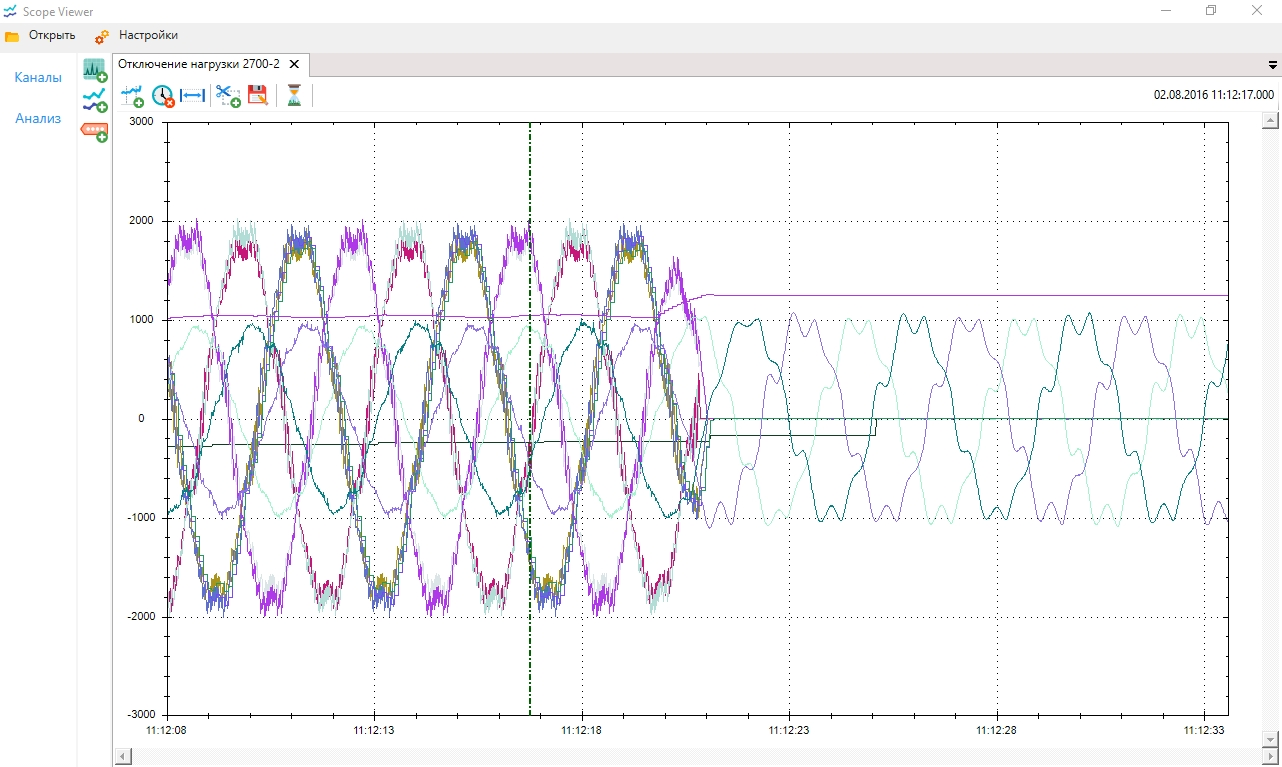
\includegraphics[width=80ex]{image/MainWindow.jpg}
\caption{Главное окно приложения.}
\end{figure}

\section*{\hspace{.5cm}Элементы управления }
\hspace{.5cm}В  верхней  части  окна  расположена  панель  инструментов,  на  которой расположены  кнопки «Открыть» и «Настройки», позволяющие открыть файл осциллограммы и настроить параметры приложения.

Слева располржены кнопки «Каналы» и «Анализ» дающие возможность настроить параметры каналов осциллограмм и просмотреть мгновеные значения. 

Между кнопками «Каналы», «Анализ» и графиком осциллограмм расположена панель дополнительных инструментов, позволяющие: добавить новый график, объеденить осциллограммы и открыть дискретный канал.

\section*{\hspace{.5cm}Настройка каналов }
\hspace{.5cm}При открытие меню «Каналы» , отоброзятся настройки каналов открытых осциллограмм. Чтобы увидеть подробную информацию о канале необходимо нажать по его названию. Ниже приведены параметры, которые можно изменить в меню настройки каналов:

\begin{enumerate}
\item - Выбор типа канала аналоговый или цифровой. 
\item - Выбор типа линии отображаймого канала: сплошная, пунктирная, точечная.
\item - Выбор типа линии отображаймого канала.
\item - Отобразить или скрыть все каналы осциллограммы на графике.
\item - Выбрать все каналы осциллограммы.
\item - Закрыть осциллограмму.
\item - Отображение отдельного канала. 
\item - Выбрать канал.
\item - Изменить цвет линии отображения канала.
\item - Включить сглаживание.
\item - Отображать канал толстой линией.
\end {enumerate}

\begin{figure}[h]
\centering
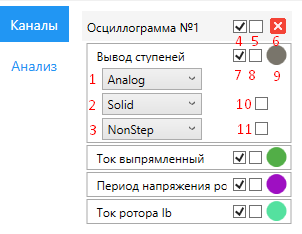
\includegraphics[width=40ex]{image/Channel.png}
\caption{Настройка каналов.}
\end{figure}

\section*{\hspace{.5cm} График осциллограммы}
\hspace{.5cm}Каждая график осциллограмм открывается в своей вкладке и имеет собственную панель инструментов. В верхнем правом углу отображается штамп времени. 

\begin{figure}[h]
\centering
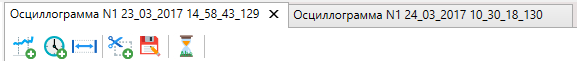
\includegraphics[width=55ex]{image/Screenshot_2.png}
\caption{Вкладки графиков осциллограмм.}
\end{figure}

Основные инструменты панели перечислены ниже.
\begin{enumerate}
\item 
\includegraphics[width=4ex]{image/Stocks_Add.png} - Добавить куросры . Для перемещения курсоров нужно нажать по нему и отпустить, после этого его можно свободно перемещать. В меню «Анализ» будут отображатся мгновенные значения каналов в положениях курсоров. 
\item 
\includegraphics[width=4ex]{image/Watch_Add.png} - Добавить штамп времени на график.
\item 
\includegraphics[width=4ex]{image/Width-48.png} - Масштабирование по горизонтали.
        
\includegraphics[width=4ex]{image/Height-48.png} - Масштабирование по вертикали. 
	  
\includegraphics[width=4ex]{image/Resize-48.png} - Масштабирование по горизонтали и вертикали.
\item 
\includegraphics[width=4ex]{image/Cutting_Add.png} - Вырезать участок осциллограммы.
	 
\includegraphics[width=4ex]{image/Cut_Apply.png} - Применить действия.
\item 
\includegraphics[width=4ex]{image/Save_as_48.png} - Сохранить осциллограмму. Осциллограмма сохраняется в формате TEXT FILE (*.txt). 
\item 
\includegraphics[width=4ex]{image/Time_abs.png} - Переключение между абсолютным и относительным временем. 
\end {enumerate}


Дополнительные инструменты панели графика осциллограмм доступны при открытом дискретном канале. Список дополнительных инструменотов представлен в следующем списке. 

\begin{enumerate}
\item 
\includegraphics[width=4ex]{image/FlipVertical.png}, 
\includegraphics[width=4ex]{image/FlipHorizontal.png}  - Расположение. Меняет расположение отображаемых графиков с вертикального на горизонтальное и наоборот.
\item 
\includegraphics[width=4ex]{image/Dig_Cancel.png} - Убрать дискретный канал. Удаляет дискретный канал с графика.
\item 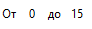
\includegraphics[width=12ex]{image/Screenshot_1.png} - Позволяет редактировать отображение дискретного канала.
\end {enumerate}

Нажав правой кнопкой мыши по вкладкам раскроется меню, в котором можно расположить графики осциллограмм вертикально или горизонтально. При закрытии графика осциллограммы закроется и осциллограмма в меню «Каналы».

\begin{figure}[h]
\centering
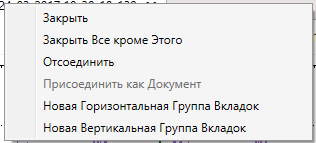
\includegraphics[width=40ex]{image/Screenshot_4.png}
\caption{Меню вкладки.}
\end{figure}

Нажав правой кнопкой мыши по самому графику откроется меню, в котором можно: копировать график в буфер обмена для последующей вставки в графический файл, сохранить график как рисунок, отправить график на печать, отображать значения точек на графике и управлять масштабом.

\begin{figure}[h]
\centering
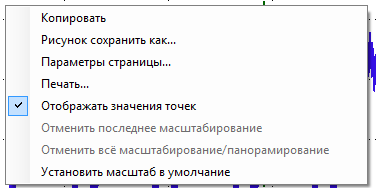
\includegraphics[width=40ex]{image/Screenshot_6.png}
\caption{Меню вкладки.}
\end{figure}

\section*{\hspace{.5cm} Дополнительные возможности}
\hspace{.5cm} Инструмент «Добавить новый график»  
\includegraphics[width=4ex]{image/Chromatography.png}  позволяет создать новую осциллограмму. Для этого необходимио выбрать интересующие каналы в меню «Каналы». 

Инструмент «Объеденить осциллограммы»  
\includegraphics[width=4ex]{image/Line_Chart.png}  позволяет объеденить каналы различных осциллограмм в одну, при условии что они следуют друг за другом. Для этого необходимио в меню «Каналы» выбрать интересующие каналы в осциллограммах. 

Инструмент «Открыть дискретный канал»  
\includegraphics[width=4ex]{image/Dig_Add.png}  позволяет раскрыть канал по битам, при этом тип рассматриваемого канала должен быть дискретный. Одновременно можно рассматривать только один дискретный канал. При открытии будет предложено выбрать дискретность канала.

\begin{figure}[h]
\centering
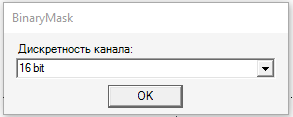
\includegraphics[width=40ex]{image/BinaryMask.png}
\caption{Дискретность канала.}
\end{figure}

\section*{\hspace{.5cm} Настройки приложения}
\hspace{.5cm} В настройкак приложения (кнопка «Настройки»  
\includegraphics[width=4ex]{image/Services-48.png}) можно настройти параметры отображаймых графиков. 

Низкий уровень детализации позволяет увеличить скорость отрисовки, но при этом теряется его качество.

Линии сетки упрощают ориентирование на графике. Можно настроить отображение  как основных, так промежуточных (вспомогательных) линии сетки.

Легенда помогает разобраться в представленных данных. Можно настроить ее отображение, размер и положение на графике.

\begin{figure}[h]
\centering
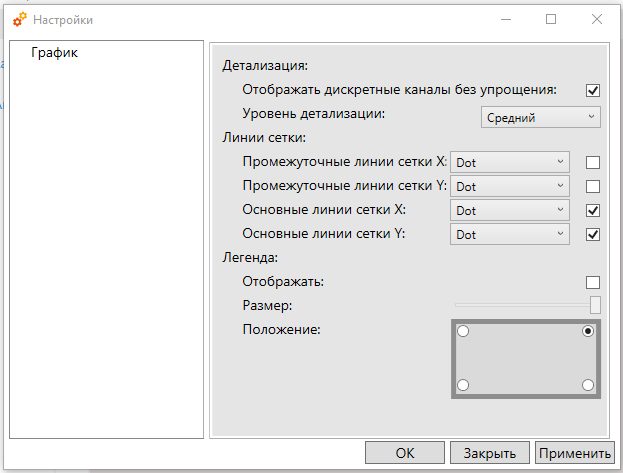
\includegraphics[width=65ex]{image/Screenshot_5.png}
\caption{Настройки приложения.}
\end{figure}

\end{document}


